\documentclass[11pt]{amsart}
\usepackage[a4paper,textwidth=158mm,textheight=237mm,centering]{geometry}
\usepackage[T1]{fontenc}
\usepackage{lmodern,microtype,mathtools,amssymb,graphicx,flafter,booktabs}
\usepackage[unicode,colorlinks=true,linkcolor=black,citecolor=black,urlcolor=blue]{hyperref}
\newtheorem{theorem}{Theorem}[section]
\newtheorem{lemma}[theorem]{Lemma}
\newtheorem{proposition}[theorem]{Proposition}
\newtheorem{corollary}[theorem]{Corollary}
\theoremstyle{definition}
\newtheorem{definition}[theorem]{Definition}
\theoremstyle{remark}
\newtheorem{remark}[theorem]{Remark}
\newcommand{\Hl}{H_{\mathrm{lat}}}
\title{Exact Heesch numbers of small edge-marked polyforms}
\author{Harvey Yorke}
\address{Valyu AI}
\ifdefined\journalversion\else
\author{Valyu DeepResearch}
\address{Valyu AI}
\fi
\ifdefined\journalversion
  \hypersetup{pdftitle={Exact Heesch numbers of small edge-marked polyforms},pdfauthor={Harvey Yorke}}
\else
  \hypersetup{pdftitle={Exact Heesch numbers of small edge-marked polyforms},pdfauthor={Harvey Yorke and Valyu DeepResearch}}
\fi
\date{26 October 2026}
\keywords{Heesch number, Heesch's problem, marked polyforms, satisfiability, DRAT certificates}
\newcommand{\paperAuthorBlock}[1]{%
  \begin{minipage}[t]{.44\textwidth}
    \centering\normalfont\normalsize #1\par\small Valyu AI\par
  \end{minipage}%
}
\makeatletter
\renewcommand{\@setauthors}{%
  \begingroup\trivlist\centering\normalfont\normalsize
  \@topsep30\p@\relax\advance\@topsep by -\baselineskip\item\relax
  \ifdefined\journalversion
    \paperAuthorBlock{Harvey Yorke}%
  \else
    \paperAuthorBlock{Harvey Yorke}\hspace{.06\textwidth}\paperAuthorBlock{Valyu DeepResearch}%
  \fi
  \endtrivlist\endgroup
}
\renewcommand{\@setaddresses}{}
\makeatother
\begin{document}
\raggedbottom
\begin{abstract}
An edge-marked polyform carries a bump, a nick or nothing on each boundary edge. When bumps and nicks are unequal in number the shape cannot tile the plane, so its Heesch number is finite. Mann showed that straight rows of $n\ge4$ hexagons with his hexapillar marking reach Heesch number $5$. A later computer search of marked polyforms stopped at five coronas. Following a suggestion of Kaplan, we encode lattice coronas of marked polyforms in propositional satisfiability (SAT), and we make the marking itself a Boolean variable. One solver call then decides whether \emph{any} unbalanced marking of a fixed base shape admits $k$ coronas. Our model uses grid-aligned copies, one centred mark per edge and strict coronas, whose unions are closed disks. In it we determine the maximum lattice Heesch number over all unbalanced markings for every polyhex with at most four cells, for the straight row of five hexagons and for every polyomino with at most five cells. No unbalanced marking of the straight four- or five-hexagon row admits six coronas. So in this model Mann's value $5$ is the best possible for these two base shapes. No polyomino with at most five cells exceeds $3$. Every lower bound comes with an explicit corona patch checked by a standard-library program. Every upper bound is the unsatisfiability of a CNF formula, certified by a DRAT proof checked with \texttt{drat-trim}. We also give an independent, replayable exact check that the six-corona patch Ba\v{s}i\'c published for his record figure satisfies the strict definition. The results are incremental. They settle small cases exactly in a direction others have explored heavily, and they do not bear on whether a Heesch number of $7$ exists.
\end{abstract}
\maketitle

\section{Introduction}

A closed topological disk $T$ that does not tile the plane has \emph{Heesch number} $k$ if $k$ is the largest integer such that $T$ can be surrounded $k$ times by congruent copies of itself~\cite{Heesch1968,GS1987}. Heesch's problem asks which values occur. The planar record is $6$, held by Ba\v{s}i\'c's figure of 2021~\cite{Basic2021}. In 2026 Ba\v{s}i\'c showed that finite Heesch numbers are unbounded in $\mathbb E^3$~\cite{Basic2026}. In the plane, $6$ remains the largest known value~\cite{Basic2026,Kaplan2025}.

Edge markings are the oldest route to high Heesch numbers. A polyform whose boundary edges carry bumps, matching nicks and flat edges, with bumps always fitting into nicks, is an \emph{edge-marked polyform}. Mann's $n$-hexapillars are rows of $n$ hexagons with a particular marking. They have Heesch number $4$ for $n=2,3$ and $5$ for $n\ge4$~\cite[Theorem~1]{Mann2004}, proved in general in his thesis~\cite{MannThesis}. Marshall independently found the value $4$ for $n=2$~\cite{Mann2004}. Mann's polypillars, the polyomino analogue, reach $3$~\cite[Theorem~2]{Mann2004}. Mann and Thomas then took a small family of low-order polyominoes, polyhexes and polyiamonds and enumerated all bump-and-nick assignments to their edges~\cite{MannThomas2016}. Kaplan's account of that search~\cite{Kaplan2022} says that it found Heesch numbers up to $5$, but the computation stopped at five coronas and left most cases inconclusive. The main obstacle was the lack of a procedure for deciding which marked shapes tile. We could not read the full text of~\cite{MannThomas2016}, so we cannot say how far its tables overlap with ours. Some of our lower bounds, and possibly some of our smaller exact values, may already be there.

Since 2019 this circle of ideas has been explored intensely. In 2019 Smith posted shapes on a grid of hexagons joined point to point, with reported Heesch numbers $4$ and $5$~\cite{SmithBlog2019}. D\v{z}uklevski describes the planar record holders with Heesch number $6$, Ba\v{s}i\'c's figure among them, as a family first found by Smith~\cite{Dzuklevski2026}. The Heesch Number Atlas~\cite{BakkerAtlas} is a website associated with Anton Bakker. It reports automated sweeps of marked tiles on eight lattices, with Heesch numbers up to $5$ for marked polyiamonds. It is unreviewed. Among its entries are the straight rows of four and five hexagons, drawn as polyiamonds of $24$ and $30$ triangles. For one marking of each row, a block of bumps followed by a block of nicks with one element more or fewer and then a single flat edge, it lists Heesch number exactly $5$. Its model is the triangular lattice, which as far as we can tell also allows placements off the hexagonal grid. Ba\v{s}i\'c, D\v{z}uklevski and Slivkov\'a survey related variants~\cite{BDS2023}. We claim no new record. Our contribution is exactness over \emph{all} markings of small base shapes, with certificates that a reader can replay.

\subsection*{Method}
Kaplan's SAT method computes Heesch numbers of unmarked polyforms~\cite{Kaplan2022}. In his conclusions he notes that the technique ``could easily be extended to handle marked polyforms, simply by prohibiting adjacencies that are not compatible with the markings''. He adds that one must then check that the markings prevent tiling, ``whether based on combinatorial imbalance or a more complex computation''~\cite{Kaplan2022}. We take the imbalance route, with one further step: the marking is not fixed in advance but is part of the SAT instance. If a marking has more bumps than nicks, no tiling exists, by the classical counting argument (Proposition~\ref{prop:realize}). A single cardinality constraint on the marking variables therefore guarantees non-tiling. One instance then asks whether \emph{some} marking with $\#\text{bumps}-\#\text{nicks}\ge1$ admits $k$ coronas, and swapping bumps and nicks covers every unbalanced marking. Balanced markings that fail to tile for other reasons are outside the method. They were the inconclusive population of the earlier search.

\subsection*{Results}
All statements concern the lattice Heesch number of Definition~\ref{def:lattice}: grid-aligned copies, one centred mark per edge, strict coronas.
\begin{itemize}
\item[(A)] For the straight rows of $4$ and of $5$ hexagons, the maximum over all unbalanced markings is exactly $5$ (Theorem~\ref{thm:bars}).
\item[(B)] The maximum for every polyhex with at most $4$ cells is given in Table~\ref{tab:hex}. The overall maximum is $5$, reached only by the straight four-hexagon row (Theorem~\ref{thm:hex}).
\item[(C)] The maximum for every polyomino with at most $5$ cells is given in Table~\ref{tab:sq}. The overall maximum is $3$, reached only by the straight rows of $4$ and $5$ squares (Theorem~\ref{thm:sq}).
\item[(D)] Ba\v{s}i\'c's published patch of $169$ tiles is a valid six-corona patch under the strict closed-disk definition (Theorem~\ref{thm:basic}).
\end{itemize}

\section{Definitions}\label{sec:defs}

We use the hexagonal grid and the square grid. Hexagons have unit distance between neighbouring centres and are given in axial coordinates, with neighbour vectors $(\pm1,0)$, $(0,\pm1)$ and $\pm(1,-1)$. A \emph{polyform} $P$ is a finite set of cells whose union is a closed disk. Its \emph{boundary edges} are the cell edges that lie on $\partial P$. A \emph{marking} is a map $\mu$ from boundary edges to $\{b,n,f\}$ (bump, nick, flat). Its \emph{imbalance} is $d(\mu)=\#\mu^{-1}(b)-\#\mu^{-1}(n)$, and the marking is \emph{unbalanced} if $d(\mu)\ne0$.

\begin{definition}[lattice coronas]\label{def:lattice}
A \emph{copy} of $(P,\mu)$ is its image under a symmetry of the grid (rotations, reflections and translations preserving the grid), with the marks carried along. Two copies are \emph{compatible} if they share no cell and every edge they share is labelled $b$--$n$, $n$--$b$ or $f$--$f$. A \emph{$k$-corona patch} is a family of pairwise compatible copies with levels $0,\dots,k$ such that:
\begin{enumerate}
\item level $0$ consists of $P$ itself;
\item every copy of level $i\ge1$ shares a boundary point with a copy of level $i-1$;
\item $U_i$, the union of the copies of level at most $i$, is a closed topological disk for every $i$;
\item $U_{i-1}$ lies in the interior of $U_i$ for $1\le i\le k$.
\end{enumerate}
The \emph{lattice Heesch number} $\Hl(P,\mu)$ is the largest $k$ for which a $k$-corona patch exists. For a base polyform $P$ let $h(P)=\max\{\Hl(P,\mu): d(\mu)\neq0\}$.
\end{definition}

Conditions (1)--(4) are Ba\v{s}i\'c's Definition~1~\cite{Basic2021}, restricted to grid-aligned copies. They give the hole-free convention behind Kaplan's $H_c$~\cite{Kaplan2022}. Condition (3) asks for a closed disk, which also excludes pinch points, not merely holes. Exchanging $b$ and $n$ on every copy preserves compatibility, so $\Hl(P,\mu)=\Hl(P,\bar\mu)$, where $\bar\mu$ swaps bumps and nicks. Hence $h(P)$ is the maximum over markings with $d(\mu)\ge1$.

Two other conventions give larger numbers and are not treated here. Kaplan's $H_h$ allows holes in the outermost corona~\cite{Kaplan2022}. Day's convention for realized shapes allows a nick to face a flat edge or another nick, which leaves a small void. Under Day's convention Ammann's marked hexagon has Heesch number $4$ instead of $3$~\cite{EppsteinJunkyard}. Our compatibility rule forbids such contacts.

\section{Realization and non-tiling}

Fix $0<r<1/4$. The \emph{realization} $T_\mu$ of $(P,\mu)$ is obtained from $P$ by two operations, both centred at edge midpoints. On each $b$ edge we attach the closed half-disk of radius $r$ lying outside $P$. On each $n$ edge we remove from $P$ the open disk of radius $r$ about the midpoint. This removes the middle edge segment as well as the inward half-disk, leaving the inward semicircle as boundary. The distance from an edge midpoint to any other grid edge is $\sqrt3/6>1/4$ for hexagons, attained at the endpoints of the edge, and $1/2$ for squares. Each half-disk therefore lies in a single cell, apart from its diameter. Half-disks in a common cell are disjoint, since midpoints of distinct edges of a cell are at least $1/2$ apart. So $T_\mu$ is a closed topological disk, and all vertices of $P$ lie on its boundary.

\begin{proposition}\label{prop:realize}
Let $d(\mu)\ne0$. Consider families of congruent copies of $T_\mu$ with pairwise disjoint interiors, under arbitrary isometries.
\begin{enumerate}
\item Let $\alpha$ be a bump arc of a copy $A$ with an interior point that is also interior to the union. Then $\alpha$ coincides with the full nick arc of exactly one other copy.
\item $T_\mu$ does not tile the plane.
\item $\Hl(P,\mu)\le H(T_\mu)<\infty$.
\end{enumerate}
\end{proposition}

\begin{proof}
(1) Let $C$ be the circle of radius $r$ carrying $\alpha$, and let $x$ be an interior point of $\alpha$ that is interior to the union. Points just outside $C$ near $x$ belong to other copies, whose boundaries near $x$ consist of segments and radius-$r$ arcs. A segment cannot follow $C$. A convex arc of another copy on $C$ would put that copy inside the disk bounded by $C$, which near $x$ belongs to $A$. So the boundary near $x$ is a nick arc $\beta$ of some copy $B$, on the same circle $C$. Suppose $\beta\ne\alpha$. Then $\beta$, a closed semicircle of $C$, contains points beyond an endpoint of $\alpha$. There $C$ runs into the interior of the cell of $A$ that carries $\alpha$, while $B$ occupies the outside of $C$ near $\beta$, so the interiors of $A$ and $B$ meet. Hence $\beta=\alpha$. Two different copies cannot both have their nick on $\alpha$, since both would occupy the outside of $C$ near $x$.

(2) Suppose the copies tile the plane. In a tiling the matching in (1) is also onto: a generic interior point of a nick arc must face a convex arc of another copy on the same circle; applying (1) to that bump gives the whole matching semicircle. Local finiteness follows from bounded tile diameter, positive tile area and disjoint interiors. Thus every bump and every nick belongs to a unique matched pair. Let the more numerous kind be the surplus arcs, with count $\beta$, and let the other kind have count $\nu$; then $\beta-\nu=|d(\mu)|\ge1$. Let $\delta$ be the diameter of $T_\mu$ and $D_R$ the disk of radius $R$ about the origin. Let $S_R$ be the set of copies contained in $D_{R-\delta}$, and $E_R$ the set of copies meeting $D_R$ but not contained in $D_{R-\delta}$. Every surplus arc of a copy in $S_R$ matches an opposite arc of a copy meeting $D_R$. Distinct surplus arcs have distinct partners, so
\[
\beta\,|S_R|\le \nu\,(|S_R|+|E_R|),\qquad\text{so}\qquad |d(\mu)|\,|S_R|\le \nu\,|E_R|.
\]
The copies have equal area and disjoint interiors. The copies in $E_R$ lie in an annulus of width $3\delta$ about $\partial D_R$, so $|E_R|=O(R)$. Likewise $|S_R|\ge cR^2$ for large $R$, because the copies meeting $D_{R-2\delta}$ cover it and all lie in $S_R$. This is a contradiction for large $R$. The argument is Epstein's counting argument for marked hexagons and Mann's $O(\sqrt n)$ bound~\cite{Mann2004}, in the area-versus-perimeter form also used by D\v{z}uklevski~\cite{Dzuklevski2026}, written for arbitrary isometries.

(3) Replace every copy in a lattice $k$-corona patch by its realization. On each shared edge either a bump fills a nick exactly or two flat edges coincide. So interiors stay disjoint, and copies that touched at a vertex or along an edge still touch, because vertices are unaffected. Each union $U_i$ changes only by disjoint half-disks attached to or removed from its boundary edges, so it remains a closed disk. Every boundary edge of $U_{i-1}$ faces a cell of $U_i$ by condition (4). By compatibility the realized marks there are a matched bump and nick or two flat edges, so $U_{i-1}$ remains in the interior of $U_i$. This gives a $k$-corona patch of $T_\mu$ in the sense of~\cite[Definition~1]{Basic2021}. Finiteness of $H(T_\mu)$ follows from (2) and the extension theorem~\cite[Section~3.8]{GS1987}.
\end{proof}

\begin{remark}
Proposition~\ref{prop:realize}(3) gives only $H(T_\mu)\ge\Hl(P,\mu)$. For the realized figure, copies that are not aligned to the grid might give more coronas, for example by sliding along flat edges or by sitting on the finer triangular lattice. Every upper bound below is a statement about $\Hl$ and not about $H(T_\mu)$. The same restriction to grid-aligned placements underlies the polyform computations of~\cite{Kaplan2022}.
\end{remark}

\section{The encoding}\label{sec:enc}

Fix $P$, its boundary edges $e_1,\dots,e_E$ and $k$. The variables are as follows:
\begin{itemize}
\item a label $L_{e,x}$ for each edge $e$ and $x\in\{b,n,f\}$, with exactly one true per edge;
\item a placement variable $u_p$ for each grid symmetry $p$ whose translation part lies in the disk of radius $\rho$ of Lemma~\ref{lem:radius};
\item level indicators $\ell_{p,j}$ and cumulative indicators $c_{p,j}$ (level at most $j$), for $0\le j\le k$;
\item cell coverage $A_{z,j}$ (cell $z$ covered at level at most $j$);
\item auxiliary variables $Y_{\pi,x}$ (the copy owning the directed edge position $\pi$ shows label $x$ there).
\end{itemize}
The constraints are:
\begin{itemize}
\item[(i)] Imbalance: the bump indicators minus the nick indicators sum to at least $1$, written as a sequential-counter cardinality constraint~\cite{PySAT}.
\item[(ii)] The identity placement has level $0$ and no other placement does. Every placement has at most one level, and every cell is covered by at most one placement.
\item[(iii)] Interior containment: $A_{z,j}\Rightarrow A_{z',j+1}$ for every cell $z'$ sharing a point with $z$ ($j<k$). These are the six edge-neighbours for hexagons and the eight neighbours for squares.
\item[(iv)] Contact: $\ell_{p,j}\Rightarrow\bigvee_{z'}A_{z',j-1}$, with $z'$ ranging over cells outside $p$ that share a point with $p$.
\item[(v)] Labels: $u_p\wedge L_{e,x}\Rightarrow Y_{\pi(p,e),x}$, and $\neg(Y_{\pi,x}\wedge Y_{\pi',y})$ for opposite positions $\pi,\pi'$ of one grid edge with $\{x,y\}$ not complementary.
\item[(vi)] A cell having a point-neighbour outside the search window (a \emph{rim cell}) may not be covered below level $k$.
\end{itemize}
We call (i)--(vi) the \emph{base formula} $F(P,k)$. Constraint (iv) asks for contact with level \emph{at most} $j-1$. This is weaker than condition (2), which is harmless for unsatisfiability claims. Witnesses are checked against the definition itself.

A satisfying assignment gives a marking $\mu$ with $d(\mu)\ge1$ and a family of copies satisfying Definition~\ref{def:lattice}, except that the unions may enclose uncovered cells. To find witnesses we add hole-blocking clauses lazily. Suppose a model leaves a bounded component $Z$ of uncovered cells inside $U_j$, with components taken under edge-adjacency. We then add $\bigvee_{p\in\mathcal B}\neg c_{p,j}\vee A_{z,j}$, where $\mathcal B$ is the set of placements of level at most $j$ touching $Z$, and $z\in Z$. This clause holds in every patch satisfying Definition~\ref{def:lattice}. If all of $\mathcal B$ is present at level at most $j$, the cells around $Z$ are covered, so an uncovered $z$ would lie in a bounded complementary component of $U_j$. These clauses are used only to find witnesses. None of our unsatisfiability claims uses them.

\begin{lemma}\label{lem:radius}
Let $(0,0)\in P$, and let $\delta$ be the largest centre-to-centre distance between cells of $P$. Let $s$ be the largest centre distance between two cells sharing a point: $s=1$ for hexagons and $s=\sqrt2$ for squares. In any $k$-corona patch, every cell of a copy of level $j$ has its centre within $R_j=\delta+j(\delta+s)$ of the origin. Hence a search window of radius $\rho\ge k(\delta+s)+2\delta+2$ loses no patch, and constraint (vi) is valid.
\end{lemma}
\begin{proof}
For $j=0$ this is the definition of $\delta$. A copy of level $j$ shares a point with a cell of level at most $j-1$. That cell lies within $R_{j-1}$, so the touching cell of the copy lies within $R_{j-1}+s$, and every other cell of the copy within a further $\delta$. Every cell with centre within $\rho$ of the origin occurs in the window: take the identity rotation and that cell as the translation. Copies of level at most $k$ have translations within $R_k\le\rho$. Cells of level below $k$ lie within $R_{k-1}$, so all their point-neighbours lie within $R_{k-1}+s\le\rho$, and none of them is a rim cell.
\end{proof}

\begin{remark}\label{rem:holes}
The base formula has no hole-blocking clauses. So its unsatisfiability also excludes patches whose unions $U_i$ enclose uncovered cells, as long as each $U_{i-1}$ lies in the interior of $U_i$. All the upper bounds below are unsatisfiability results for base formulas. This relaxation keeps the compatibility rule, so it is neither Kaplan's $H_h$ nor Day's convention.
\end{remark}

\section{Results}

\begin{theorem}\label{thm:bars}
Let $B_n$ be the straight row of $n$ hexagons. Then $h(B_4)=h(B_5)=5$. Equivalently, with one centred mark per edge and grid-aligned copies, no unbalanced marking of $B_4$ or $B_5$ admits six coronas.
\end{theorem}

\begin{proof}[Evidence]
Lower bound: explicit five-corona patches with imbalance $+1$, of $131$ copies for $B_4$ and $157$ copies for $B_5$, pass the independent checker (Section~\ref{sec:cert}). Upper bound: the base formulas $F(B_4,6)$ and $F(B_5,6)$ are unsatisfiable. Their sizes and the DRAT checks are listed in Table~\ref{tab:drat}.
\end{proof}

Mann's Theorem~1~\cite{Mann2004} gives a specific marking of $B_n$, the hexapillar, with Heesch number $5$ for $n\ge4$. For $n=4,5$, Theorem~\ref{thm:bars} says that in the lattice model no unbalanced marking of the same base shape does better. We could not compare our optimal markings with Mann's Figure~5 in detail. Our optimal markings agree with those listed in the Heesch Number Atlas, up to exchanging bumps and nicks.

\begin{figure}[ht]
 \centering
 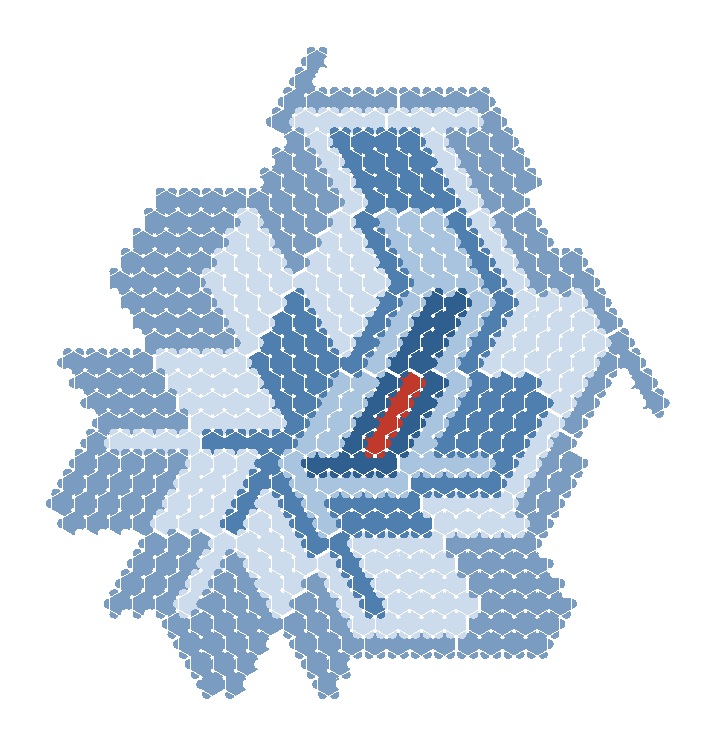
\includegraphics[width=.62\textwidth]{patch-bar4.pdf}
 \caption{A five-corona patch of $131$ copies of the straight four-hexagon row (centre, red), marked cyclically with nine bumps, one flat edge and eight nicks. Coronas alternate in shade; bumps are drawn as half-disks and sit in the matching nicks. By Theorem~\ref{thm:bars} no unbalanced marking of this row admits a sixth lattice corona.}
 \label{fig:patch}
\end{figure}

\begin{theorem}\label{thm:hex}
The values $h(P)$ for all twelve free polyhexes with at most four cells are those in Table~\ref{tab:hex}.
\end{theorem}

\begin{theorem}\label{thm:sq}
The values $h(P)$ for all twenty-one free polyominoes with at most five cells are those in Table~\ref{tab:sq}. In particular no unbalanced marking of a polyomino with at most five cells admits four lattice coronas.
\end{theorem}

\begin{table}[ht]
\centering\small
\caption{Exact values $h(P)$ for polyhexes with at most four cells and the straight row of five, in axial coordinates (neighbours $(\pm1,0)$, $(0,\pm1)$, $\pm(1,-1)$). ``Copies is the size of the witness patch; the last three columns describe the unsatisfiable base formula $F(P,h+1)$.}\label{tab:hex}
\begin{tabular}{lrrrrr}\toprule
base cells & $h$ & copies & $k$ refuted & variables & clauses\\\midrule
$(0,0)$ & 3 & 37 & 4 & 21\,147 & 97\,591 \\
$(0,0),\,(1,0)$ & 4 & 81 & 5 & 148\,738 & 842\,676 \\
$(0,0),\,(0,1),\,(0,2)$ & 4 & 64 & 5 & 354\,150 & 2\,300\,354 \\
$(0,0),\,(0,1),\,(1,-1)$ & 3 & 40 & 4 & 186\,413 & 1\,215\,829 \\
$(0,0),\,(0,1),\,(1,0)$ & 2 & 19 & 3 & 62\,216 & 380\,082 \\
$(0,0),\,(0,1),\,(0,2),\,(0,3)$ & 5 & 131 & 6 & 947\,735 & 6\,895\,353 \\
$(0,0),\,(0,1),\,(0,2),\,(1,-1)$ & 2 & 25 & 3 & 218\,300 & 1\,606\,698 \\
$(0,0),\,(0,1),\,(0,2),\,(1,0)$ & 3 & 37 & 4 & 241\,059 & 1\,665\,581 \\
$(0,0),\,(0,1),\,(1,-2),\,(1,-1)$ & 2 & 19 & 3 & 217\,718 & 1\,605\,756 \\
$(0,0),\,(0,1),\,(1,-1),\,(1,0)$ & 2 & 20 & 3 & 121\,330 & 801\,306 \\
$(0,0),\,(0,1),\,(1,-1),\,(1,1)$ & 1 & 6 & 2 & 82\,057 & 614\,375 \\
$(0,0),\,(1,-2),\,(1,-1),\,(2,-1)$ & 1 & 7 & 2 & 68\,989 & 514\,805 \\
$(0,0),\,(0,1),\,(0,2),\,(0,3),\,(0,4)$ & 5 & 157 & 6 & 1\,562\,333 & 12\,387\,835 \\
\bottomrule\end{tabular}
\end{table}

\begin{table}[ht]
\centering\small
\caption{Exact values $h(P)$ for polyominoes with at most five cells. Columns as in Table~\ref{tab:hex}.}\label{tab:sq}
\begin{tabular}{lrrrrr}\toprule
base cells & $h$ & copies & $k$ refuted & variables & clauses\\\midrule
$(0,0)$ & 1 & 9 & 2 & 5\,417 & 21\,243 \\
$(0,0),\,(0,1)$ & 2 & 23 & 3 & 42\,184 & 200\,356 \\
$(0,0),\,(0,1),\,(0,2)$ & 2 & 26 & 3 & 94\,530 & 503\,460 \\
$(0,0),\,(0,1),\,(1,0)$ & 1 & 6 & 2 & 33\,641 & 177\,031 \\
$(0,0),\,(0,1),\,(0,2),\,(0,3)$ & 3 & 50 & 4 & 288\,869 & 1\,717\,113 \\
$(0,0),\,(0,1),\,(0,2),\,(1,0)$ & 2 & 21 & 3 & 115\,664 & 674\,996 \\
$(0,0),\,(0,1),\,(0,2),\,(1,1)$ & 1 & 8 & 2 & 54\,859 & 313\,963 \\
$(0,0),\,(0,1),\,(1,-1),\,(1,0)$ & 1 & 6 & 2 & 62\,171 & 358\,935 \\
$(0,0),\,(0,1),\,(1,0),\,(1,1)$ & 1 & 7 & 2 & 36\,629 & 194\,175 \\
$(0,0),\,(0,1),\,(0,2),\,(0,3),\,(0,4)$ & 3 & 51 & 4 & 463\,951 & 2\,960\,137 \\
$(0,0),\,(0,1),\,(0,2),\,(0,3),\,(1,0)$ & 1 & 10 & 2 & 110\,009 & 679\,287 \\
$(0,0),\,(0,1),\,(0,2),\,(0,3),\,(1,1)$ & 1 & 6 & 2 & 101\,205 & 623\,499 \\
$(0,0),\,(0,1),\,(0,2),\,(1,-1),\,(1,0)$ & 1 & 9 & 2 & 108\,969 & 677\,411 \\
$(0,0),\,(0,1),\,(0,2),\,(1,0),\,(1,1)$ & 1 & 8 & 2 & 67\,287 & 387\,975 \\
$(0,0),\,(0,1),\,(0,2),\,(1,0),\,(1,2)$ & 1 & 7 & 2 & 68\,149 & 418\,107 \\
$(0,0),\,(0,1),\,(0,2),\,(1,0),\,(2,0)$ & 1 & 8 & 2 & 92\,809 & 576\,207 \\
$(0,0),\,(0,1),\,(0,2),\,(1,1),\,(2,1)$ & 1 & 8 & 2 & 68\,041 & 417\,891 \\
$(0,0),\,(0,1),\,(1,-1),\,(1,0),\,(2,-1)$ & 1 & 8 & 2 & 93\,601 & 577\,827 \\
$(0,0),\,(0,1),\,(1,-1),\,(1,0),\,(2,0)$ & 1 & 8 & 2 & 67\,521 & 416\,903 \\
$(0,0),\,(0,1),\,(1,0),\,(2,-1),\,(2,0)$ & 1 & 7 & 2 & 93\,721 & 578\,031 \\
$(0,0),\,(1,-1),\,(1,0),\,(1,1),\,(2,0)$ & 1 & 9 & 2 & 59\,049 & 363\,699 \\
\bottomrule\end{tabular}
\end{table}


\begin{figure}[ht]
 \centering
 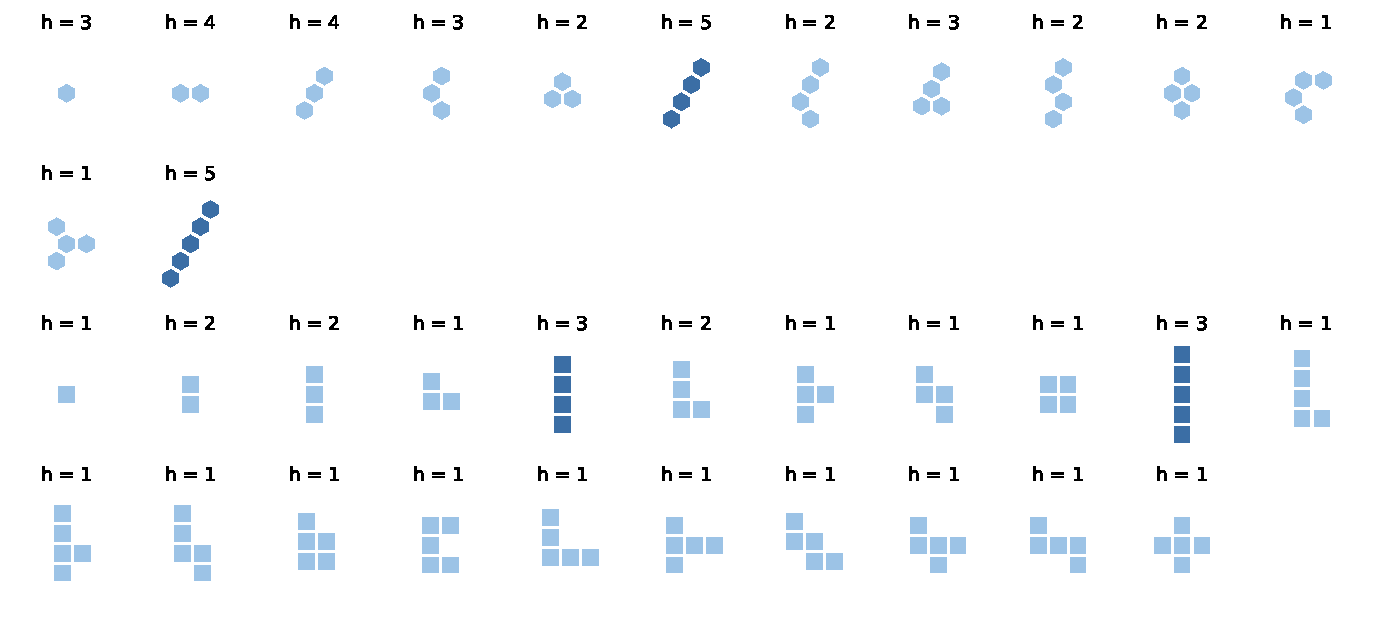
\includegraphics[width=\textwidth]{table-tiles.pdf}
 \caption{The base shapes of Tables~\ref{tab:hex} and~\ref{tab:sq} with their values $h$; the maximum in each class is shaded darker.}
 \label{fig:tiles}
\end{figure}

The values for the straight rows agree with Mann's theorems: $h=4$ for the rows of $2$ and $3$ hexagons, and $h=2,2,3$ for the rows of $2,3,4$ squares~\cite{Mann2004}. Those theorems concern particular markings, whereas $h$ maximizes over all markings. For the single hexagon, $h=3$ is already known. Epstein's counting proof, reported by Mann~\cite{Mann2004}, shows that no unbalanced marked hexagon has Heesch number above $3$: a fourth corona would hold $61$ tiles but have only $54$ boundary edges for their surplus bumps. Mann also notes that the markings of a single hexagon can simply be enumerated~\cite{Mann2004}. For the longer base shapes such counting bounds are not sharp, and the exclusions come from the solver.

\begin{remark}[shape of the optimal markings]
Read around the boundary, the marking in each of our optimal witnesses for the straight rows $B_1,\dots,B_5$ has the same form. It consists of a block of $m+1$ bumps, one flat edge and a block of $m$ nicks, where $2m+2$ is the number of boundary edges. The straight-row witnesses have imbalance $1$, agreeing with the Atlas's empirical observation about deep markings. Six witnesses for other bases have imbalance $2$ or $3$; no general imbalance-one theorem is asserted. For comparison, see~\cite{BakkerAtlas}. We did not determine whether other markings are also optimal.
\end{remark}

\begin{remark}[two marks per edge]
Our encoders also allow $m$ marks per edge: slot $i$ of one side faces slot $m-1-i$ of the other, and reflections reverse the order. Such off-centre marks are not covered by Proposition~\ref{prop:realize}. With $m=2$ and imbalance $1$ the solver found no five-corona patch for the domino of hexagons. We report this as a solver result only, without a DRAT proof. It is not part of the theorems.
\end{remark}

\section{Ba\v{s}i\'c's six-corona patch}\label{sec:basic}

Ba\v{s}i\'c's figure is the union of six regular hexagons, eleven equilateral triangles and half an equilateral triangle, arranged on the trihexagonal ($3.6.3.6$) grid. His paper shows a patch of $169$ copies in six coronas. It explains that every copy in a surround must follow the grid lines, so a computer search becomes feasible and confirms that $6$ is the maximum~\cite{Basic2021}. We parsed the vector drawing of that figure on Wikimedia Commons~\cite{BasicSVG}. The drawing is credited to Ba\v{s}i\'c and to the published paper, and it was uploaded by a third party. Every one of its $169$ polygons snaps to a grid-aligned copy of the figure, with a largest vertex deviation of $0.002$ grid units after scaling. We recorded the copies exactly on the grid of hexagons and drafters, the six $30$-$60$-$90$ pieces of each triangle. The corona sizes are $1,6,10,13,32,52,55$.

\begin{theorem}\label{thm:basic}
The snapped integer patch satisfies Definition~\ref{def:lattice}(1)--(4) for Ba\v{s}i\'c's figure with $k=6$, with every copy aligned to the refined grid. Every union $U_i$ is a closed disk: edge-connected, a manifold at every vertex, with Euler characteristic $1$. Each $U_{i-1}$ lies in the interior of $U_i$.
\end{theorem}

The theorem confirms a published claim. It adds no new fact about the figure, but it gives an exact certificate that anyone can replay. The Heesch Number Atlas lists Ba\v{s}i\'c's figure as re-verified at Heesch number $6$. It also notes that its own stored six-corona witness has a pinch point and that a strict witness of its own was still being sought~\cite{BakkerAtlas}. The published patch, read off the drawing, has no pinch point.

\section{Certificates}\label{sec:cert}

\emph{Witnesses.} Every lower bound in Tables~\ref{tab:hex} and~\ref{tab:sq} is a JSON file of explicit copies, given as integer matrices and translations. The checker \texttt{check\_marked.py} uses only the Python standard library and integer arithmetic. From the definitions alone, it verifies lattice symmetry, disjointness, label compatibility, contact, the disk property of every $U_i$, interior containment and $d(\mu)\neq0$. The disk property is checked through edge-connectivity and Euler characteristic, and directly by requiring the boundary edges to form one connected cycle with degree two at every boundary vertex. This last test rejects holes, disconnected components and pinch points. The Ba\v{s}i\'c patch is additionally checked by this boundary-cycle test at all seven levels, independently of the original checker's vertex-fan test (with the same exact geometric representation). Mutated witnesses are rejected. A separate exact checker on the refined trihexagonal grid checks Ba\v{s}i\'c's patch.

\emph{Upper bounds.} Each upper bound $h(P)<k$ rests on the base formula $F(P,k)$, which the encoder regenerates deterministically; its SHA-256 hash is recorded. We solved each formula with CaDiCaL~3.0.1~\cite{CaDiCaL}, writing a binary DRAT proof, and checked the proof with \texttt{drat-trim}~\cite{DRATtrim}. The proofs are not shipped because of their size. Their hashes are recorded. Two runs of one small formula with CaDiCaL~3.0.1 produced bit-identical proofs. The regeneration commands and original hashes are supplied, but bit identity has not been tested for every formula. A different valid proof is acceptable only after a fresh replay against the matching CNF. The default build checks retained verification logs and does not rerun the DRAT checker. We did not use a formally verified proof checker.

\emph{Encoding cross-checks.} DRAT certifies that a formula is unsatisfiable, not that it encodes Definition~\ref{def:lattice}. We checked the encoding in three ways. First, a second encoder builds cells, edges and contacts from polygon vertices instead of axial offsets. It agrees with the first on every value of Tables~\ref{tab:hex} and~\ref{tab:sq}, at $k=h$ and at $k=h+1$, except the two large formulas of Theorem~\ref{thm:bars}. Both encoders implement the same specification, so this checks the implementation, not the specification. Second, the encoder reproduces the known values: $3$ for the single hexagon, Mann's hexapillar values $4,4,5,5$ and his polypillar values $2,2,3$. Third, with every edge forced flat and the imbalance constraint removed, the encoder computes Heesch numbers of unmarked polyforms. On 41 saved non-tiling polyhex cases of sizes six and seven, its values $H_c$ agree with Kaplan's independently written \texttt{heesch-sat}. For example the base $\{(0,0),(1,-1),(2,-2),(3,-2),(4,-2),(4,-1)\}$ has $H_c=2$ in both implementations. The retained case-by-case outputs are checked by \texttt{check\_crosschecks.py}; this is an implementation control, not an exhaustive classification at those sizes.

\begin{table}[ht]
\centering\small
\caption{The largest refuted formulas. Times are wall-clock on a shared, heavily loaded laptop; all other formulas are smaller and are listed in \texttt{results.json}.}\label{tab:drat}
\begin{tabular}{lrrrrr}\toprule
base cells & $k$ & clauses & CaDiCaL (s) & proof (GB) & drat-trim (s)\\\midrule
$(0,0),\,(0,1),\,(0,2),\,(0,3)$ & 6 & 6\,895\,353 & 3\,920 & 0.3 & 3\,446 \\
$(0,0),\,(0,1),\,(0,2),\,(0,3),\,(0,4)$ & 6 & 12\,387\,835 & 8\,597 & 0.7 & 4\,379 \\
\bottomrule\end{tabular}
\end{table}


\section{Scope and limitations}

\begin{itemize}
\item The upper bounds concern grid-aligned copies, one centred mark per edge and strict coronas. Richer alphabets (several marks per edge, colours, oriented edges) are not covered, and neither are copies off the grid, holes in the outermost corona or Day's void-permitting convention. Under oriented matching rules an unpublished Heesch number of $11$ is reported~\cite{BDS2023}.
\item Only unbalanced markings are covered. A balanced marking that does not tile could in principle do better. The method has no non-tiling certificate for such markings.
\item Mann--Thomas~\cite{MannThomas2016} may already contain some small-table entries; their full text was unavailable. Our all-markings exclusion at six coronas goes beyond the five-corona cut-off reported by Kaplan. The Atlas already lists $5$ for one marking of each straight row~\cite{BakkerAtlas}. Priority for the maximum over all unbalanced markings remains subject to this bibliographic limitation.
\item The method does not approach the open question of a planar figure with Heesch number $7$~\cite{Kaplan2025,BakkerAtlas}.
\end{itemize}

\bibliographystyle{plain}
\bibliography{references}
\end{document}
